\documentclass{article}

\usepackage{graphicx}
\usepackage{amsmath}
\usepackage{amsthm}
\usepackage{float}
\usepackage{hyperref}
\usepackage[margin=1.25in]{geometry}

\theoremstyle{plain}
\newtheorem{definition}{Definition}
\newtheorem{theorem}{Theorem}
\newtheorem{lemma}{Lemma}
\newtheorem{corollary}{Corollary}

\title{Security on Networks}
\date{\today}
\author{Bonny Jain, John Wang, Iris Xu}

\begin{document}

  \maketitle

\section{Introduction}

As epidemics spread on computer, disease propagation, and financial networks, agents in the network often undertake costly investments in security to protect themselves from infection. However, these investments are often imperfect and typically succeed with some probability less than one. Furthermore, the cost of a security investment and its probability of success both increase with the chosen level of security. Thus agents face a tradeoff between choosing high investment in security to minimize infection probability and choosing low investment to minimize cost. Given the easily definable utility functions of agents, it is appropriate to model the choice of security as a game on a network.

In this paper, we extend the game theoretic framework developed in unpublished work from Acemoglu et al. to random graph models. We spend the majority of the paper considering the static model of infection in which each agent chooses a security level once before epidemic propagation. In the static infection model, we specifically concern ourselves with characterizing the difference in infection rates between the Nash equilibrium and the social optimum. We also discuss some simulation results on the dynamic model, in which agents observe the infection state of their $k$-neighborhood at each timestep and update their security investments accordingly. Finally, we present some results on the intractability of computing infection probabilities exactly, and we provide a fully polynomial time approximation scheme for arbitrarily small $\epsilon$.

\section{Static Infection Model}

Although modeling infection on the network dynamically with a model such as SIR is more representative of real epidemics, such a model is intractable for the purpose of theoretical reasoning. In this section, we utilize the static model of infection as described in unpublished work by Acemoglu et al. (2013). Specifically, we apply the network security game model to Erd\H{o}s-R\'{e}nyi random graphs. We characterize the difference in network infection rates between the case of actions chosen by rational utility-maximizing agents and the case of actions chosen to maximize total social welfare. This difference is significant, as it can be readily interpreted as the cost of anarchy in a society with interactions modeled by a random graph. 

\subsection{Game Definition}

The game proceeds on a network $A$ drawn from the set of Erd\H{o}s-R\'{e}nyi random graphs on $n$ nodes with edge probability $p$. Before the network is sampled from the ER graph distribution, each agent makes a security investment $q_i \in [0, 1]$, knowing only the values of $n$ and $p$, such that agent $i$ is immunized against infection at the beginning of the game with probability $q_i$. Agent $i$ incurs a cost $c(q_i)$ by choosing security level $q_i$, and we define all agents to have identical cost functions that are positive, strictly increasing, and strictly convex. 

A random attacker then chooses one of the $n$ agents uniformly at random and exposes this agent to infection. If the chosen agent $i$ is not immunized, the infection spreads to all susceptible agents on the component of agent $i$. We define $\textbf{P}(A, \textbf{q})$ to be the probability of infection of agent $i$ on random graph $A$ when the agents collectively play security profile $\textbf{q}$. The utility function of agent $i$ is given by:
\begin{eqnarray}
	u_i(q_i) = -\textbf{P}(A, \textbf{q}) - c(q_i)
\end{eqnarray} 
We define $\tilde{\textbf{P}}(A,q_{-i})$ to be the probability that agent $i$ is exposed to infection given that all other agents play security profile $q_{-i}$. Then, using a result from Acemoglu et al., we can rewrite the utility function as:
\begin{eqnarray}
	u_i(q_i) = -(1-q_{i})\tilde{\textbf{P}}(A,q_{-i}) - c(q_i)
\end{eqnarray}
Next, we define social welfare $W(\textbf{q})$ to be the sum of the utilities of all agents, namely:
\begin{eqnarray}
	W(\textbf{q}) = \sum\limits_{i \in A} u_i(q_i) = \sum\limits_{i \in A}  -(1-q_{i})\tilde{\textbf{P}}(A,q_{-i}) - c(q_i)
\end{eqnarray}
In the case of a Nash equilibrium, each agent chooses $q_i$ to maximize his utility function given that the remaining agents collectively play $q_{-i}$. In the case of the social optimum, each agent chooses $q_i$ to maximize social welfare given $q_{-i}$.

\subsection{Erd\H{o}s-R\'{e}nyi Framework}

As we will discuss later, computing infection probabilities and equilibria is not computationally feasible for general networks. However, Erd\H{o}s-R\'{e}nyi random graphs are a subset of a class of networks defined by Acemoglu et al. termed symmetric networks, whose properties we can exploit to allow computation of equilibria. A random network $A$ is defined as a symmetric network if for any permutation of the vertices $\pi : V \rightarrow V$, $\pi(A)$ has the same distribution as $A$. Clearly, Erd\H{o}s-R\'{e}nyi graphs belong to this category of networks. We will utilize the following theorem Acemoglu et al. that characterizes equilibria in symmetric networks.
\begin{theorem}
	Suppose all agents have positive, increasing, and convex cost functions. Then, on a symmetric network, there exist a unique symmetric equilibrium profile $q^e$ and a unique symmetric social optimum $q^s$, and $q^e \leq q^s$.
\end{theorem}
Next, we consider the importance of phase transitions in the spread of infection on the network. We recall that there are three significant phases in an ER graph - in Phase I, $p < \frac{1}{n}$, in Phase II, $\frac{1}{n} < p < \frac{\log{n}}{n}$, and in Phase III, $p >  \frac{\log{n}}{n}$. The transition between Phase I and Phase II corresponds to the emergence of a giant component, and the transition between Phase II and Phase III corresponds to the vanishing of all other components. The first phase transition is very important in our analysis, since the emergence of a giant component yields a transition to a positive probability of infection. The second phase transition, however, corresponds to a vanishing of a few leftover isolated nodes and small components. This transition does not affect the probability of infection in a discontinuous manner, and therefore we model the phases of the network simply as subcritical (Phase I) and supercritical (Phases II and III).

\subsection{Equilibrium and Social Optimum}

First, we consider the Nash equilibrium and social optimum in the subcritical case, i.e. when there exists no giant component. Since $qn$ of the agents are immunized at the beginning of the game, the effective size of the remaining network is $n(1-q)$.Therefore, the network exists in the subcritical phase for $(n(1-q)-1)p < 1$. Let $S(q, n)$ denote the expected size of the component of a randomly chosen node. The following equation is adapted from Equation (4.19) in Jackson, derived using a generating function argument.
\begin{eqnarray}
	S(q, n) = 1 + \frac{1}{1 - (n(1-q)-1)p}
\end{eqnarray}
The expected probability that infection reaches any node is given by $\frac{S(q, n)}{n}$. Then, for large $n$, we have $\tilde{\textbf{P}}(A,q_{-i}) \rightarrow 0$. Thus, the utility and social welfare functions reduce to:
\begin{equation}
	u_i(q_i) = -c(q_i)
\end{equation}
\begin{equation}
	W(q) = -nc(q)
\end{equation}
Maximizing the left-hand sides for both of the equations above gives us $q^e = q^s = 0$ for the subcritical case. 

Next, we consider the supercritical case, i.e. when a giant component exists. The probability of infection on a component smaller than the giant component is vanishingly small for large $n$, so we shall restrict our attention to infection on the giant component. The probability of exposure of agent $i$ to infection in the supercritical case is the probability that the initial attack is delivered to a node in the giant component and that agent $i$ is located in the giant component. Since each of the above events occurs with probability $s(q, n)$, we can write the probability of exposure to infection as $\tilde{\textbf{P}}(A,q_{-i}) = s(q, n)^2$, where $s(q, n)$ is the size of the giant component defined as a fraction of the total number of nodes. We characterize $s(q, n)$ by adapting equation 12.15 from Newman to our model:
\begin{equation}
	1 - s = e^{-(n(1-q)-1)ps}
\end{equation}
Computing an analytical solution to this equation is extremely difficult, so we will determine $s(q, n)$ numerically. 

Now, we will determine the Nash equilibrium and social optimum in the supercritical phase. We can write the utility function of agent $i$ as:
\begin{equation}
	u_i(q_i) = -(1-q_i)s(q_{-i},n)^2 - c(q_i)
\end{equation}
Differentiating both sides with respect to $q_i$ to maximize, we obtain:
\begin{equation}
	\frac{\partial u_i}{\partial q_i} = s(q_{-i},n)^2 - c'(q_i) = 0
\end{equation}
Invoking Theorem 1, we note that in equilibrium, $q^e = q_i = q_{-i}$, so our equilibrium is given by:
\begin{equation}
	c'(q^e) = s(q^e, n)^2
\end{equation}
The social welfare, which we know from Theorem 1 to be achieved by a symmetric social optimum profile, is given by:
\begin{equation}
	W(q) = -n(1-q)s(q,n)^2 - nc(q)
\end{equation}
Since we do not have a convenient closed-form expression for $s'(q, n)$, we express $q^s$ as:
\begin{equation}
	q^s = \arg\max\limits_{q\in[0,1]}\{-n(1-q)s(q,n)^2 - nc(q)\}
\end{equation}
Calculation of both $q^e$ and $q^s$ from equations (10) and (12) is performed numerically.
\subsection{Infection Rates and the Cost of Anarchy}
We define the infection rate $I(q)$ to be the expected fraction of infected nodes when all nodes play security profile $q$. The cost of anarchy is defined to be $I(q^e) - I(q^s)$, which can be intuitively regarded as the excess infection rate induced by a society of selfish utility optimizers relative to a society of agents governed by a central social welfare optimizer. Security difference is simply defined as $q^s - q^e$. 

In this section, we present numerical results on the cost of anarchy and security difference as a function of the edge probability $p$ for various cost functions. Figures \ref{cost_of_anarchy_q^2.fig}, \ref{cost_of_anarchy_sqrt(1-q^2).fig}, and \ref{cost_of_anarchy_-q-log(1-q).fig} show simulation results for various cost functions when $n=10^8$.

\begin{figure}[h!]
  \centering
  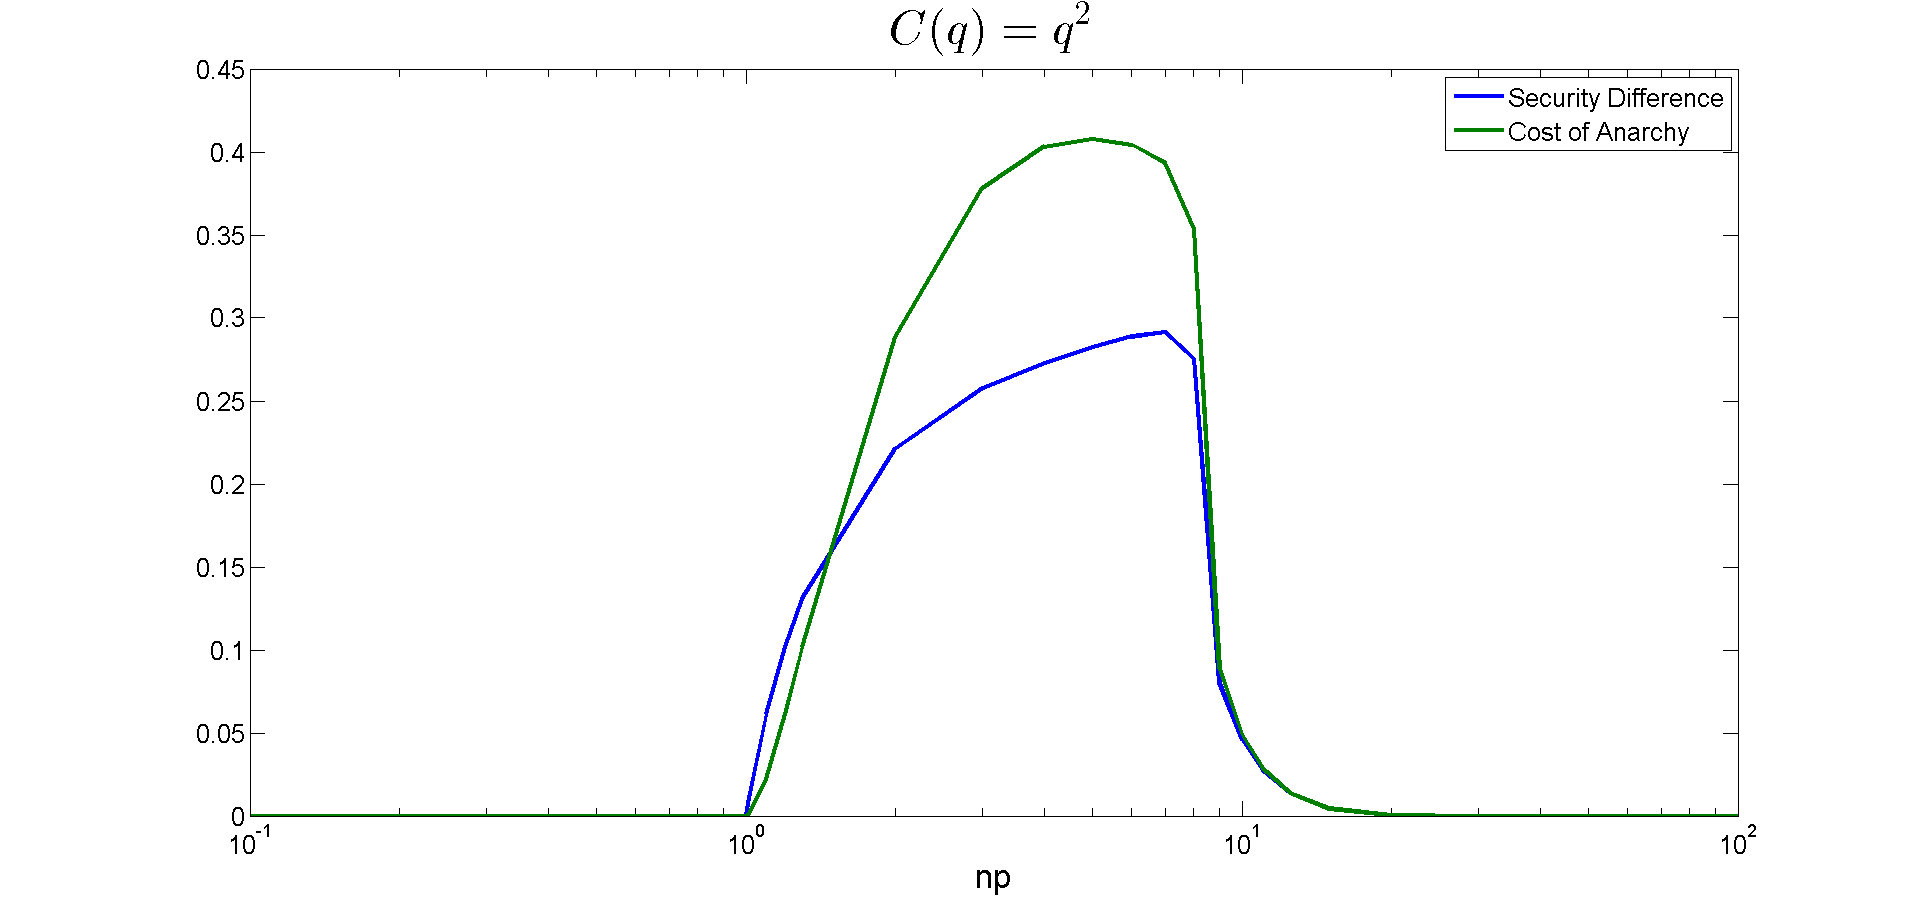
\includegraphics[width=6in]{cost_of_anarchy_q^2.png}
  \caption{Cost of Anarchy: $c(q) = q^2$}
  \label{cost_of_anarchy_q^2.fig}
\end{figure}

\begin{figure}[h!]
  \centering
  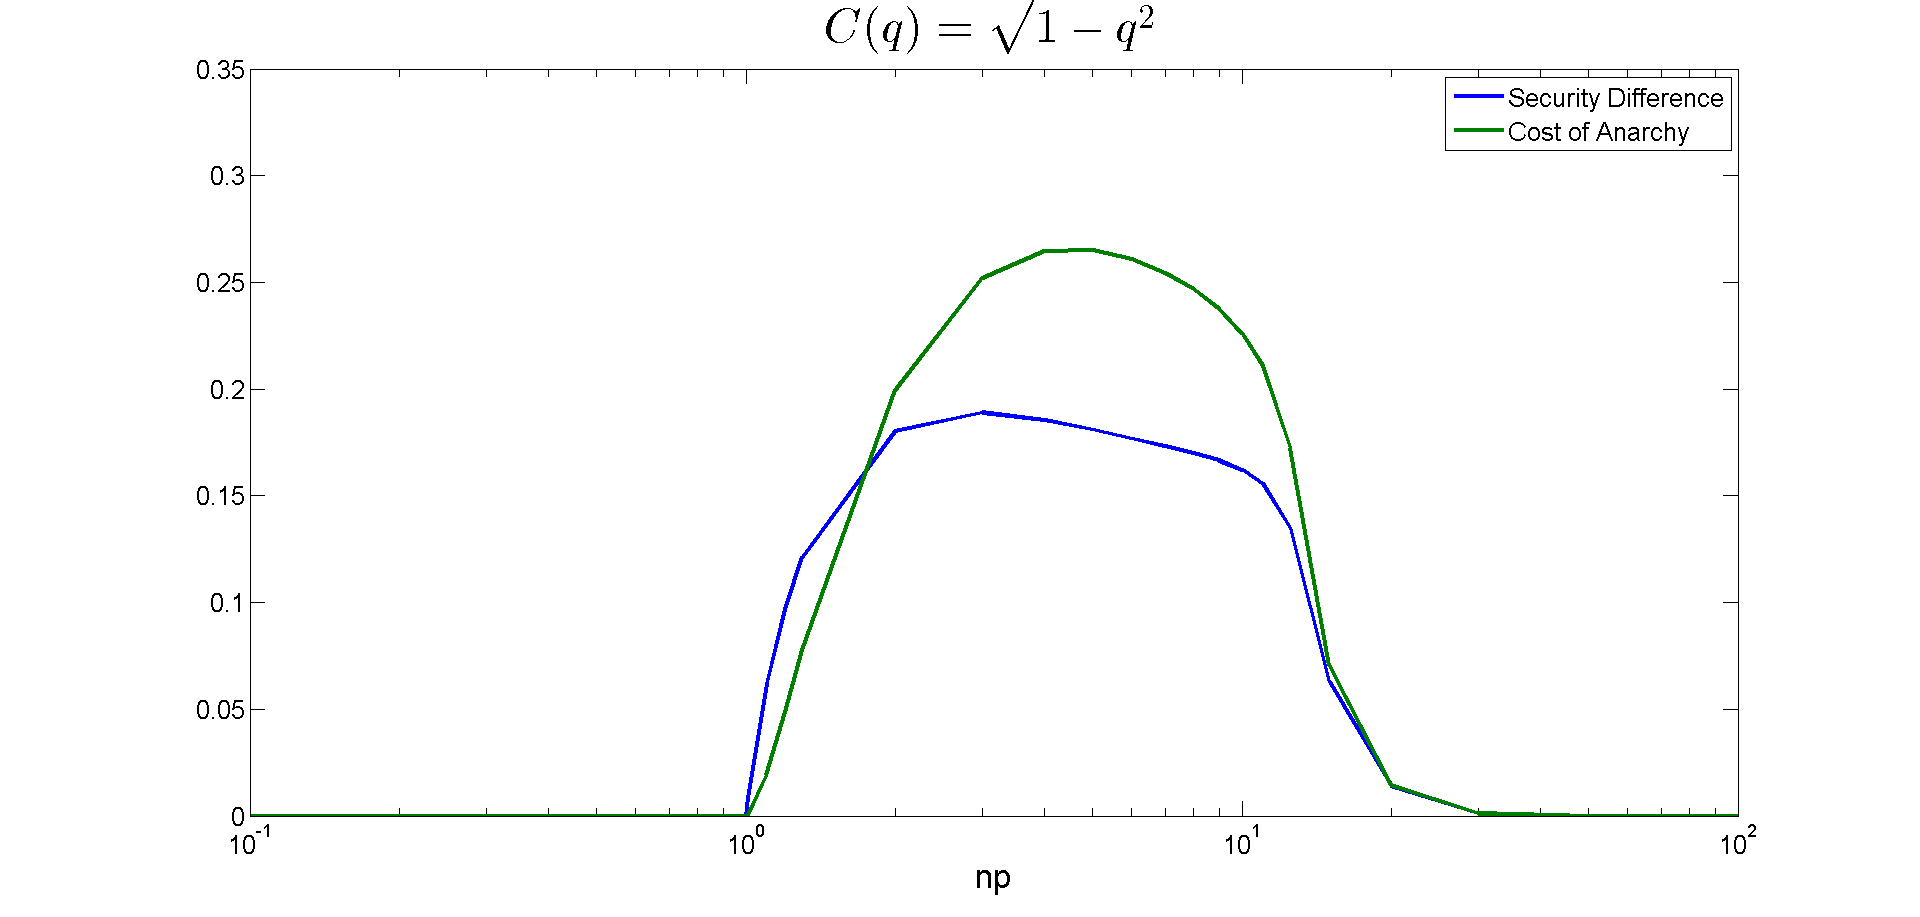
\includegraphics[width=6in]{cost_of_anarchy_sqrt(1-q^2).png}
  \caption{Cost of Anarchy: $c(q) = \sqrt{1-q^2}$}
  \label{cost_of_anarchy_sqrt(1-q^2).fig}
\end{figure}

\begin{figure}[h!]
  \centering
  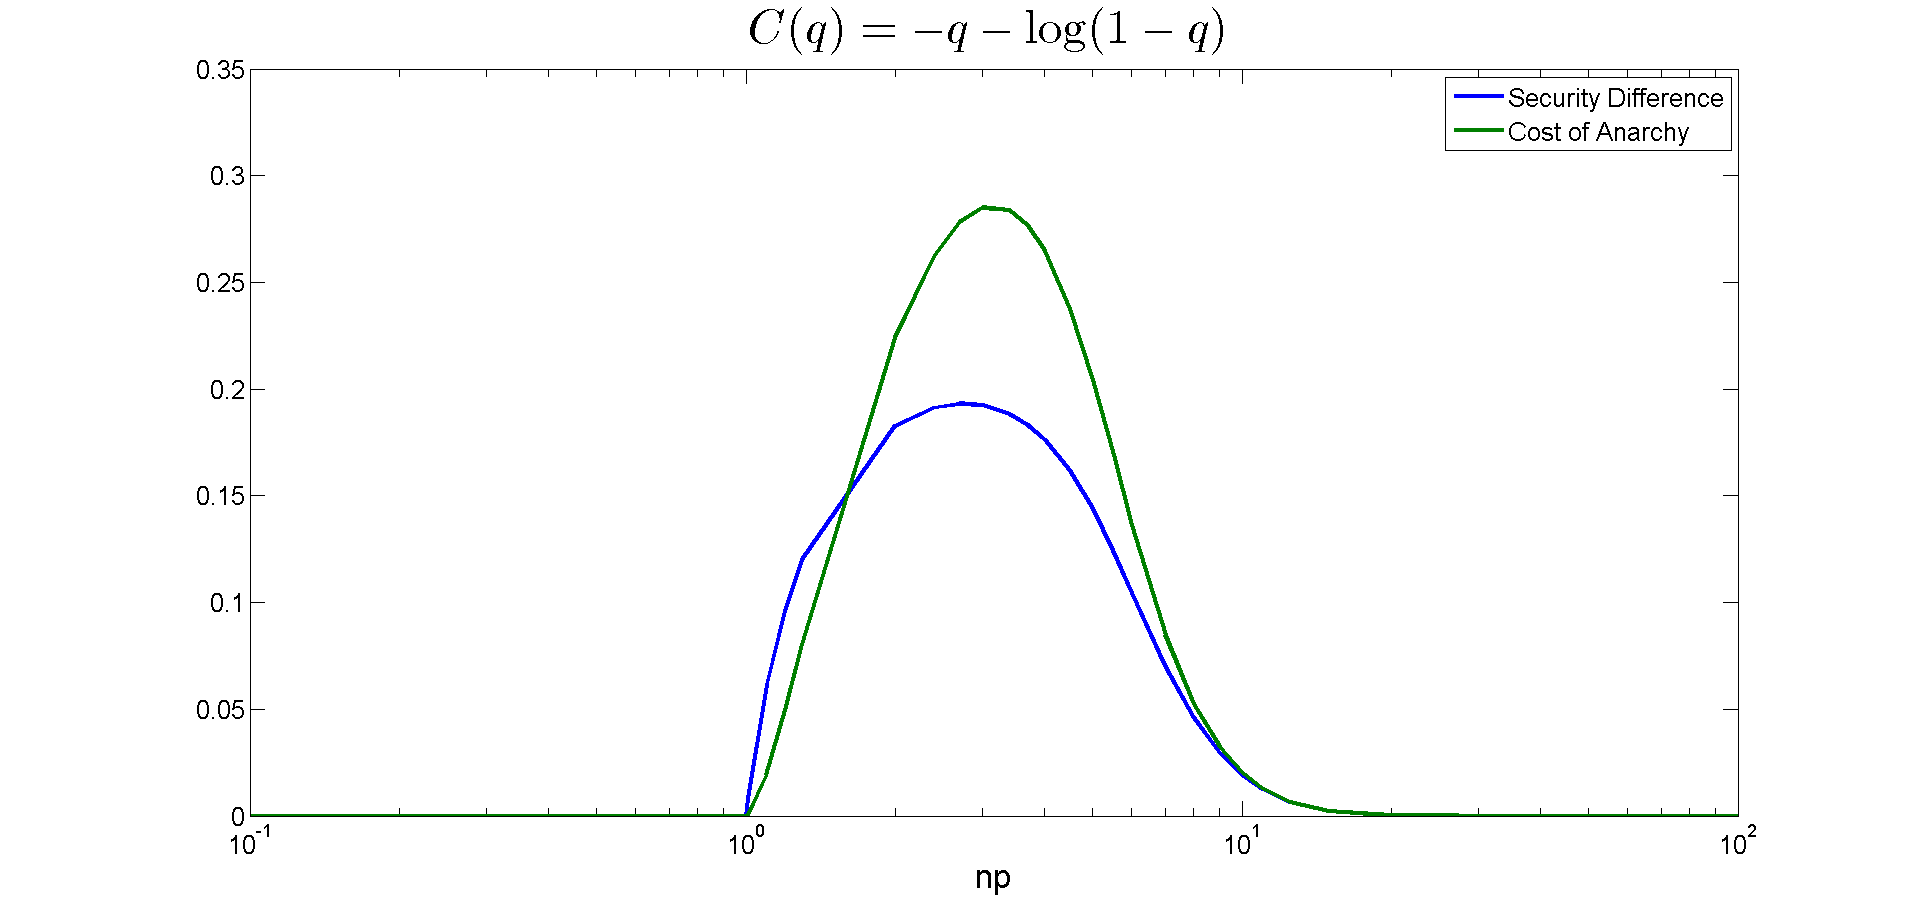
\includegraphics[width=6in]{cost_of_anarchy_-q-log(1-q).png}
  \caption{Cost of Anarchy: $c(q) = -q - \log{1-q}$}
  \label{cost_of_anarchy_-q-log(1-q).fig}
\end{figure}

For all cost functions, the cost of anarchy is exactly $0$ for subcritical probabilities, since $q^e = q^s = 0$. We also note that for $p > \frac{\log{n}}{n}$,  $\tilde{\textbf{P}}(A,q_{-i}) \rightarrow 1$, so the equilibrium and social optimum strategies converge again. Thus, it is in Phase II that the cost of anarchy is maximized. For several cost functions, the maximum cost of anarchy on a graph with $10^8$ nodes is achieved for $1<np<10$.

\section{Simulation Results}

In this section, we provide results from computational simulations of our model. The graphs that we simulate on are created using the Erdos-Renyi mechanism with the number of nodes fixed at $n = 100$. Fixing the number of nodes reduces the number of parameters that can vary.

\subsection{Simulating the Static Model}

Solving for a mixed strategy Nash Equilibrium in this context is $PPAD$ complete \cite{daskalakis08}. This implies that for all practical purposes, solving for a Nash Equilibrium is computationally intractable, although little is known about the actual complexity of $PPAD$ in relation to $P$ and $NP$ \cite{chen06}.

Because we cannot compute the equilibrium vector of protections $\bar{q}$ where $q_i \in [0,1)$ is player $i$'s choice of protection, we can sweep along a grid of representative values for $\bar{q}$ and examine the game at each one of these values.

Fortunately, this game is symmetric for each player and Acemoglu et al (2013) have shown that under such situations, the Nash Equilibrium for each player is to play the same protection $q$. Therefore it suffices to check setting $q_i = q_j$ for each player $i \neq j$ in our simulations. We shall call $q = q_i$ the protection that each player chooses.

To examine the outcome of a contagion spreading on an Erdos Renyi graph with edge probability $p$, $n = 100$, and protection rate $q$ for each participant, we must be able to compute $\tilde{P}_i(A, q_{-i}, \Phi)$, the probability that the infection reaches $i$ (i.e. the probability that any one of $i$'s neighbors gets infected). However, since computing $\tilde{P}_i$ is NP-hard, we instead use Monte Carlo simulations to approximate $\tilde{P}_i$. We do so in the following manner:

\begin{itemize}
  \item Generate $\kappa$ Erdos Renyi graphs with parameters $G(n, p)$.
  \item For each graph instance and protection value $q$, we run the following for $\gamma$ trials: choose a random node to infect and run the infection to completion.
  \item Compute $\hat{P}$, an estimate of $\tilde{P}_i$ for all $i$, as the total number of infected nodes after $\gamma$ trials divided by the total number of nodes. For $n = 100$, if we let $I_j$ be the number of infected nodes on the $j$th trial, we have:
    \begin{eqnarray}
      \hat{P} = \frac{1}{n \gamma} \sum_{j=1}^{\gamma} I_j
    \end{eqnarray}
  \item Compute the standard deviation of $\hat{P}$ by using standard techniques of computing standard deviations for a sample of random variables from a binomial distribution.
\end{itemize}

In fact, there are provable bounds on how good our Monte Carlo results are for the approximation of $\tilde{P}_i$, given by Karp and Luby (1985) for the All Terminal problem (but can easily be extended to our problem). See \cite{karp-luby85} for the full proof.

\begin{theorem}
  To estimate the probability $\tilde{P}_i$ for $i \in V \setminus u$ where $u \in V$ is the source node of the infection to within a multiplicative factor of $1 + \epsilon$ for all $\epsilon \in [0,1]$, it suffices to run the Monte Carlo algorithm for a number of trials given by:
  \begin{eqnarray}
    O \left( \frac{\ln n}{\epsilon^2 \tilde{P}_i} \right)
  \end{eqnarray}
\end{theorem}

\subsection{Static Simulation Results}

We use the above model to simulate results, with $n = 100$, $\gamma = 250$, and $\kappa = 100$. In order words, we generate $\kappa = 100$ random graphs for each set of Erdos Renyi parameters, then on each graph, we run $\gamma = 250$ distinct infections which each start at a random node. The results are then summarized for different protection rates of $q$.

We begin by presenting the average infection probability $\hat{P}$ when the edge creation probability in Erdos Renyi is very small (we choose $p = 0.005$). Here the Erdos Renyi parameter is $np = 0.5$, which is below the threshold value for the existence of a giant component. Under this regime, the average infection probability $\hat{P}$ is very low for all protection levels (even a protection rate of $q = 0.05$), as seen in the simulation results from figure \ref{avg_prob_np05.fig}.

The intuition behind this is clear. Since $np = 0.5 < 1$, the average size of a component is small, so the amount that the infection can spread is decreased. Thus, even for low protection rates, the infection cannot spread very far.

\begin{figure}[h!]
  \centering
  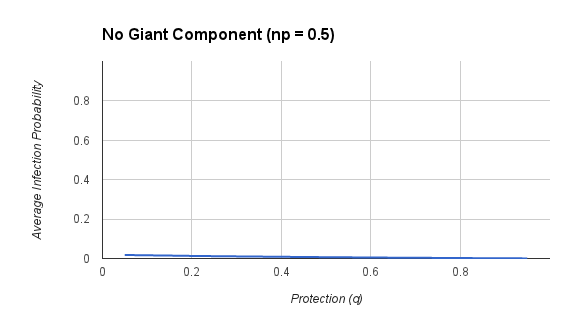
\includegraphics[width=4in]{avg_prob_np05.png}
  \caption{Average Infection Rates with No Giant Component $np = 0.5 < 1$}
  \label{avg_prob_np05.fig}
\end{figure}

When the Erdos Renyi parameter predicts the presence of a giant component, the average infection rate has a strong dependence on the protection rate. We use $np = 5 > 1$ which should produce a giant component with high probability, and simulate the resulting infection probabilities for various values of $q$. Figure \ref{avg_prob_np5.fig} shows the results from our simulations for $np = 5$. For low $q$, the average infection rate is incredibly high. For example, when $q = 0.05$, the average infection rate is $\hat{P} = 0.93$ with a standard deviation of $0.0103$.

As the protection rate increases, the average infection probability decreases almost linearly until about $q = 0.6$. Once $q = 0.6$, the positive externalities start to kick in and the average infection probability drops off more dramatically than the linear trend would predict. This can be attributed to the "network effect", or the extra benefit that everyone obtains from one person increasing their protection. Having higher $q$ will positively impact your neighbors because of the lower probability of you getting infected and thus transmitting to your neighbors. 

\begin{figure}[h!]
  \centering
  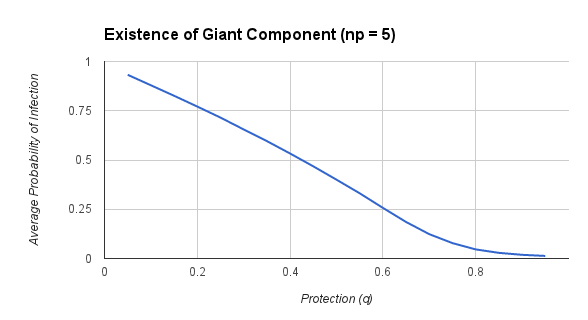
\includegraphics[width=4in]{avg_prob_np5.png}
  \caption{Average Infection Rates with Giant Component $np = 5 > 1$}
  \label{avg_prob_np5.fig}
\end{figure}

However, you must have enough connections in order for this network effect to become substantial. This is why the network effect does not manifest itself when there is no giant component. Figure \ref{network_effects_np5.fig} shows the network effect for different levels of $q$, where network effect $\nu$ is defined as follows:
\begin{eqnarray}
 \nu = 1 - q - \hat{P}
\end{eqnarray}

The network effect starts to increase to something significant by $q = 0.5$, then falls off again after $q = 0.8$. The fall off in the network effect comes from the saturation of protection levels. After a certain point, the marginal benefit of extra protection starts to decrease because of the difficulty of actually spreading the infection.

\begin{figure}[h!]
  \centering
  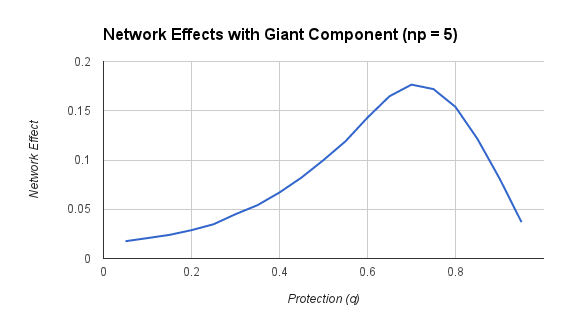
\includegraphics[width=4in]{network_effects_np5.png}
  \caption{Network Effect in a Giant Component ($np = 5$)}
  \label{network_effects_np5.fig}
\end{figure}

\subsection{Simulating the Dynamic Model}

We analyze agents dynamically choosing security. Similar to the SIR model introduced in class, we present the notion of attacking and curing nodes as agents choose their level of security at each timestep. We begin by using an Erd\H{o}s-R\'{e}nyi graph. However, in some applications, as with the case with the spread of infectious disease, the Barbasi-Albert preferential attachment model may be preferable for a higher clustering coefficient and may better mimic the choice of selecting a new partner. In the preferential attachment model with a parameter $k$, we start with $k$ nodes that are completely connected. For each node added to the graph, we add $k$ edges, weighted by the degrees of the current nodes in the graph.

Agents are fully informed of the attack and cure probabilities, as well as the security levels chosen by the nodes in their neighborhood in the previous timestep. The attack probability is equivalent to the infection rate $\alpha$ in the SIR model, i.e. the probability that a currently uninfected node will be infected at the next timestep. Similarly, the cure probability is analogous to the recovery rate $\gamma$, i.e. the probability that a currently infected node will no longer be infected at the next timestep.

At each time step, each agent chooses its level of security based on the levels of security of its neighborhood from the previous round and the attack and cure probabilities. The neighborhood of a node is defined for a pre-determined scope, indicating how deep into the graph an agent can see. For example, a scope of $1$ indicates that  agent $i$ can only view the choices of its neighbors and a scope of $2$ means that it can also see the choices of its neighbor's neighbors.

For dynamic simulations, we use a default cost function of $c(q) = q^2$. Given that the cure probability is $\gamma$ and the attack probability is $\alpha$, the probability $\tilde{\textbf{P}}(A,q_{-i})$, given the network $A$ and the security profile $q_{-i}$, that the infection reaches agent $i$ is:
\begin{equation}
	\tilde{\textbf{P}}(A,q_{-i}) = 1 - (1 - \alpha) \prod_{n \in N(i)}{(1-P_n)}
\end{equation}
where $P_n$ is the probability of the infection reaching its neighbor. For a scope of $1$, because the agent can only see a certain scope through the graph, it assumes that if it is infected, it will be no longer infected by the next time step by the cure probability and that if it is not infected, it will be infected with a probability of the attack probability. For larger scopes, the node also uses information about its neighbor's neighbors to determine the probability that infection will reach it.

\subsection{Dynamic Simulation Results}

We find that in the dynamic model, the initial choice of protection level for all of the nodes makes little difference in the resulting infection probability of the graph (Fig. \ref{fig:attack_cure}. Intuitively, this makes sense, since over many timesteps where players update their choice of protecti)on, it will converge to some relatively stable security profile, with changes from attacks and cures canceling. The results suggest that in the long-term, if attack and cure probabilities remain stable, a population of the graph will remain infected, the size of which depends on the choices of $\gamma$ and $\alpha$.

We consider the real-world application of the spread of HIV in sub-Saharan Africa. We choose to use the prevalence of HIV as the attack probability, as a measure of the invasiveness of HIV. We use the probability of death from HIV as the cure probability; because there is no current actual cure for HIV, we choose the probability of death as a measure of how often an infected node is removed from the graph. From online HIV statistics, we decide to use $\alpha=0.05$ and $\gamma=0.06$, with a preferential attachment model, and a scope of $1$. Our results suggest that in the long-term, given stable $\alpha$ and $\gamma$, a proportion of the population will always remain infected (Fig. \ref{fig:hiv}). It may seem reasonable to vary the cure probability, given that, in application, a government agent may have more control over government spending for research for a cure or other means of removing infection from the graph, whereas $\alpha$ is more likely determined by some exogenous factor. We vary $\gamma$ while fixing $\alpha=0.05$ and find that, as would be expected, infection probability decreases with increased $\gamma$, suggesting that there may be some way to predictably control infection by varying $\gamma$.

\begin{figure}[h!]
  \centering
  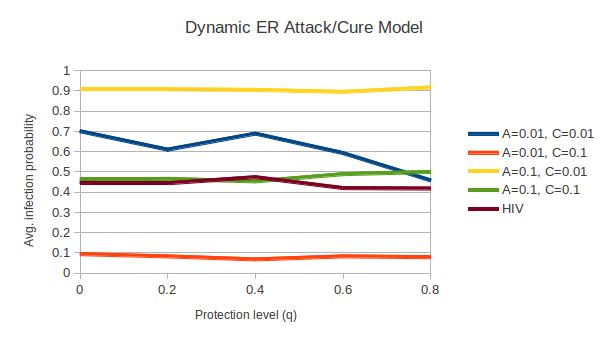
\includegraphics[width=4in]{dynamic_er_attack_cure_model.jpg}
  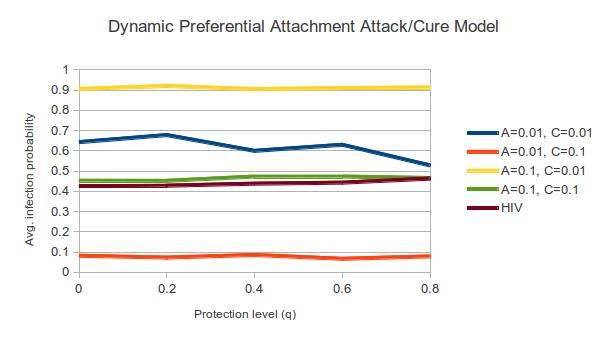
\includegraphics[width=4in]{dynamic_preferential_attachment_attack_cure_model.jpg}
  \caption{Dynamic security profile selection in the attack/cure model on a) an Erd\H{o}s-R\'{e}nyi graph and b) on a Barbasi-Albert preferential attachment graph.}
  \label{fig:attack_cure}
\end{figure}

\begin{figure}[h!]
  \centering
  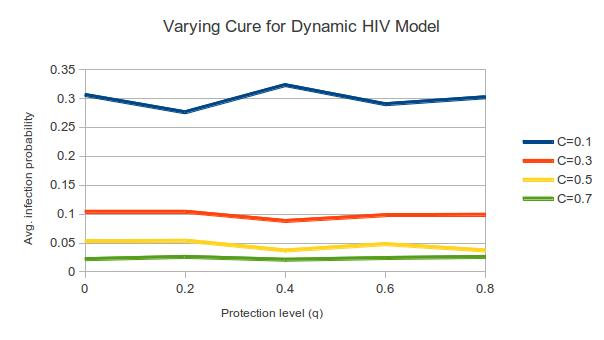
\includegraphics[width=4in]{varying_cure_for_dynamic_hiv_model.jpg}
  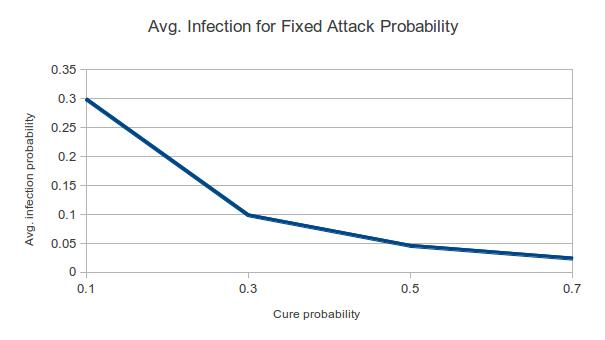
\includegraphics[width=4in]{avg_infection_for_fixed_attack_probability.jpg}
  \caption{$\alpha$ is fixed for the HIV model at $0.05$, with preferential attachment, and $\gamma$ is varied. a) shows the average infection probability for different initial protection levels and b) averages the infection probability over the different protection levels and compares to the choice of $\gamma$.}
  \label{fig:hiv}
\end{figure}


\section{Computational Intractibility Results}

Many of the critical parts required to simulate interesting scenarios of our model are NP hard. Unfortunately, this makes providing a broad range of simulation results difficult. In this section, we show a number of problems are NP hard, but also develop a polynomial time approximation scheme for computing infection probabilities.

\subsection{Computational Intractibility of $\tilde{P}_i$}

Computing $\tilde{P}_i(A, q_{-i}, \Phi)$ in general for a graph which is not a tree is in $\# P$, which is as least as hard as $NP$. This makes computing $\tilde{P}$ computationally intractable.

The reduction can be seen by introducing a known $\# P$ problem called the Two Terminal Problem.

\begin{definition}
  Let us define a graph $G = (V, E)$ with some probability labelling $Pr: E \to [0,1] \cap \mathrm{Q}$. Let $u \in V$ be a source terminal and $v \in V \setminus \{u\}$ be a target terminal. An instance of the \emph{Two Terminal Problem} is to compute $Pr(v | u)$, the probability that there exists a path to node $v$ from node $u$.
\end{definition}

Note that in the Two Terminal Problem, each edge $e \in E$ has some probability of failure $p_e \in [0,1]$ as defined by the function $Pr$.

Showing the difficulty of the computation of $\tilde{P}_i$ in the static model is now as simple as showing a reduction of the Two Terminal Problem, since it is $\# P$ complete as shown by Ball (1980) \cite{ball80}.

\begin{theorem}
  Computing $\tilde{P}_i(A, q_{-i}, \Phi)$ for all $i \in \{1, \ldots, n\}$ on an Erdos Renyi graph with edge probability $p$ is $\# P$ hard in the static model.
\end{theorem}
\begin{proof}
  We shall show that every instance of the Two Terminal Problem is an instance of the Epidemic Probability Problem (what we shall call the problem of computing $\tilde{P}_i$ in our model).

  Suppose we have an instance $\pi_{ttp}$ of the Two Terminal Problem. We can find a solution as follows:
  \begin{itemize}
    \item Create an instance $\pi_{epp}$ of the Epidemic Probability Problem using graph $G$ from $\pi_{ttp}$.
    \item Set the protection rates $q_e \in [0,1)$ for each edge $e \in E$ for the Epidemic Probability Problem as $1 - Pr(e)$, where $Pr(e)$ is the loss probability for edge $e$ in the Two Terminal Problem.
    \item Solve the Epidemic Probability Problem. The probability $\tilde{P}_v$ for a given source of infection $u$ will be the solution to the Two Terminal Problem.
  \end{itemize}

  Thus, we have shown that the Two Terminal Terminal problem can be reduced in polynomial time to the Epidemic Probability Problem, which shows that the Epidemic Probability Problem is at least as hard as the Two Terminal Problem (which is $\# P$ hard).
\end{proof}

The complexity result can be extended to the dynamic case when the protection for each node potentially changes. This means that for both the static and the dynamic model, the computation of $\tilde{P}_i$ is computationally intractable.

\begin{corollary}
  Computing $\tilde{P}_i(A, q_{-i}, \Phi)$ for all $i \in \{1, \ldots, n\}$ on an Erdos Renyi graph with edge probability $p$ is $\# P$ hard is the dynamic model with changes in protection in each time step.
\end{corollary}
\begin{proof}
  We can reduce the Two Terminal Problem to the Dynamic Epidemic Probability Problem, where the probabilities are fixed to represent $Pr$ from the Two Terminal Problem. Using the same derivation as before, we can show that the dynamic version of the Epidemic Probability Problem is $\# P$ hard.
\end{proof}

\subsection{Computationally Intractable Problems}

There are a number of related problems which are computationally hard. Actually, most interesting quantities related to the epidemic problem are NP-hard to compute. For example, computing the expected number of infected nodes is NP-hard.

\begin{theorem}
  Computing the expected number of infected nodes on the an epidemic network with protections $q_i$ for $i \in \{1, \ldots, n\}$ is $\# P$ hard.
\end{theorem}
\begin{proof}
  We shall reduce the Epidemic Probability Problem to the Epidemic Expected Infection Problem (the problem of computing the expected number of infected nodes in an epidemic network).

  Suppose we have an instance of the Epidemic Probability Problem. Now select a node $u \in V$ and create a new node $v \not \in V$ which will be attached to the graph. Now, create an edge $e(u,v)$ between $u$ and $v$ and set $v$'s protection to $q = 0$. Now, if $u$ is ever infected, then $v$ will also be infected.

  It is clear that the expected number of infected nodes in this new graph increases by $P_i(u)$, the probability of $u$ becoming infected. Thus, finding the expected number of infected nodes is at least as hard as finding the probability of infection of a node. Thus, we see that the Epidemic Expected Infection Problem is harder than the Epidemic Probability Problem, which is in $\# P$.
\end{proof}

Even the attacker's choice of target, on a general graph, cannot be computed with efficiency.

\begin{theorem}
  Computing the node to attack in order to have the highest expected number of infected nodes is NP hard.
\end{theorem}
\begin{proof}
  There is a direct bijection of this problem to the influence maximization problem, which has been shown to be NP hard by Kempe, Kleinberg, Tardos (2003) \cite{kempe-kleinberg-tardos03}.
\end{proof}


\subsection{Fast FPTAS for Infection Probabilities}

Although the problem of solving for infection probabilities is $\# P$ hard, it is still possible to approximate the probabilities. In fact, Karger (1999) developed a Fully Polynomial Time Approximation Scheme (FPTAS) for solving the all terminal problem, which can be defined as follows: given a graph $G = (V,E)$ and a probability function on the edges $Pr: E \to [0,1]$ of the probability of any edge failing, find the probability that the entire graph remains connected after edge failures occur with probability $Pr(e)$ for each edge $e \in E$.

An FPTAS is an incredibly strong result, as it means that for any $\epsilon > 0$, one can use the FPTAS to approximate the result to within a factor of $1 + \epsilon$ in time polynomial in the inputs and $\epsilon$. Thus, one can get arbitrarily close to the exact result by using a smaller and smaller $\epsilon$, in exchange for a higher running time.

There exists a naive generalization of Karger's FPTAS to the problem of computing all infection probabilities. In this section, we provide an overview of Karger's FPTAS, it's naive generalization to computing multiple-source multiple-sink infection probabilities (MSMSIP), and finally an asymptotically faster FPTAS than the naive algorithm for MSMSIP.

\subsection{Multiple-Source Multiple-Sink Infection Probabilities}

First we define the problem of computing infection probabilities for multiple sources and multiple sinks.

\begin{definition}
    We will be given a graph $G = (V,E)$ and some function of protections $Q: E \to [0,1)$ which defines the protection $q_v$ inherent for the infection to move down edge $(u,v)$. The \emph{MSMSIP problem} is to find the probability of infection $P_i(u)$ for each node $i \in V \setminus u$ for all possible starting nodes $u \in V$.
  \end{definition}

  Since we have shown the single-source single-sink infection probability problem to be $\# P$, it must be the case that MSMSIP is also $\# P$ because solving the MSMSIP implies that you have also solved the singular problem.

\subsection{Summary of Karger's FPTAS for the All Terminal Problem}

Karger solves the all terminal problem using a combination of a minimum cut finding algorithm and the Monte Carlo scheme. If $\tilde{P}_i$ is large, then it is sufficient to use the Monte Carlo algorithm because of the time bound of $O(\log n / (\epsilon^2 \tilde{P}))$. However, when $\tilde{P}$ is small and arbitrarily close to zero, the Monte Carlo simulation requires a prohibitive number of trials. Therefore, Karger develops another polynomial time algorithm which can be used when $\tilde{P} < 1/n^4$ (for explanation, we assume that all nodes have protection rate $q$, but this can be extended to each node having different protection rates without much difficulty). When this is the case, we can find cuts that are small enough, and these cuts will provide an easy way to estimate the probability of failure.

To make this argument more rigorous, we shall develop the theory more formally. Notice that graphs become disconnected exactly when all the edges in a cut fail. Thus, it is clear that if each edge $i$ in a cut fails with probability $q_i$, then the cut will fail with probability $\prod_i q_i = q^c$. Karger proves the following useful lemma.

\begin{lemma}
  Suppose $c$ is the weight of the minimum cut and an $\alpha$-minimum cut is any cut with weight less than or equal to $\alpha c$, then there are at most $n^{\alpha c}$ $\alpha$-minimum cuts.
\end{lemma}

Karger (1999) also shows that when the probability of the minimum cut failing is small, then we only need to determine the probability that a cut of value close to $c$ fails. The paper proceeds to show that it is sufficient to find the all $\alpha$-minimum cuts, of which there are $O(n^{\alpha c})$ using Karger's Recursive Contraction Algorithm. The paper shows that when $\tilde{P} < 1/n^4$, then choose:
\begin{eqnarray}
  \alpha = 2 - \frac{\ln \epsilon}{\delta \ln n}
\end{eqnarray}

Where we define $\tilde{P}^c = n^{-(2 + \delta)}$. Using this $\alpha$, Karger (1999) shows that one can find the $n^{2 \alpha}$ smallest cuts to find an $\epsilon$ approximation. To do this, we take the $n^{2 \alpha}$ smallest cuts (found using the Recursive Contraction Algorithm), and convert it into a disjunctive normal form (DNF) counting problem, which has a well-known FPTAS. Converting the set of smallest cuts into the DNF problem can be achieved by assigning a boolean variable $x_e$ to each edge $e$ and writing the probability of infecting everyone as as $F = \vee_i (\wedge_{e \subset E_i} x_e)$ for all cuts $E_i$ that we have found. Here, we let $x_e$ denote the probability of infection spreading on edge $e$. This is exactly a DNF counting problem and can be solved using Karp, Luby, and Madras's FPTAS to solve this in $O(c n^{2 \alpha} / \epsilon^2) = O(c n^4 / \epsilon^3)$ time.

\subsection{Naive Extension to MSMSIP Problem}

Using Karger (1999)'s algorithm, it is easy to take a naive approach to obtain an FPTAS for the MSMSIP problem. This can be done by first solving the single-source single-sink problem, then solving the problem for all ${n \choose 2}$ pairs of nodes, which is still a polynomial in $n$. This should provide the probability of infection for each possible pair of source infection nodes, and the second node.

To solve the single-source single-sink problem, one needs to find cuts that separate nodes $u,v$ where $u \in V$ is the source and $v \in V \setminus u$ is the sink. Karger (1999) shows in lemma 4.2 that using the same overall FPTAS structure as before, but instead solving for the smallest cuts that separate $u$ and $v$, one can achieve an FPTAS for the single-source single-sink problem. This will still have running time $O(c n^4 / \epsilon^3)$ because the Recursive Contraction Algorithm can be trivially modified to find cuts that separate $u$ and $v$.

Thus, an FPTAS to the MSMSIP problem can be achieved in ${n \choose 2} O(c n^4 / \epsilon^3) = O(c n^6 /\epsilon^3)$ running time.

\subsection{Improvements to the Naive FPTAS for MSMSIP}

However, the naive extension of Karger's FPTAS can be improved. In the following, we present a novel scheme for improving the asymptotic runtime, since $O(c n^6 / \epsilon^3)$ is probably intractable in practice. We improve the runtime of a FPTAS for MSMSIP to $O(c n^4 / \epsilon^3)$ which is potentially tractable in practice. We do this by modifying the Recursive Contraction Algorithm to find all minimum cuts and storing them.

The problem with the naive scheme is that it wastes potential information which might be useful. For example, the minimum cut between nodes $u$ and $v$ will also be the minimum cut between either $u$ or $v$ and another node $w$. This is true because there will be at least one other node in either $u$ or $v$'s partition. Note that the size $|U|$ of $u$'s partition $U$ can be related to $|V|$, the size of $v$'s partition $V$, by the expression $n = |U| + |V|$. Thus, even if $U$ only contains a single element, $V$ will contain $n-1$ elements. This simple exercise has shown that there is a large amount of repeated information between minimum cuts computed for different nodes.

In fact, we can show that one can find all the minimum cuts using the Recursive Contraction Algorithm in the same time that it takes to find a single minimum cut. Karger and Stein (1996) show that the probability $P(n)$ of a specific cut is given by $P(n) = O(1/ \ln n)$. 

\begin{theorem}
Using the Recursive Contraction Algorithm, one can find all min cuts with probability of missing any min cut at $O(1/n)$ in a running time of $O(n^2 \ln^3 n)$.
\end{theorem}
\begin{proof}
Running the Recursive Contraction Algorithm takes $O(n^2 \ln n)$ time, as described by Karger and Stein (1996), so it takes $O(n^2 \ln^3 n)$ time to run the algorithm $O( \ln^2 n)$ times. It remains to be shown that running the algorithm $O(\ln^2 n)$ times will bound the probability of missing any minimum cut by $O(1/n)$.

We know however that there are at most ${n \choose 2}$ min cuts, because each min cut must contain two partitioned sets of vertices. Moreover, the probability of not finding a specific cut $k$ is given by:
\begin{eqnarray}
  Pr[\textrm{miss }k] = (1 - P(n))^{O( \ln^2 n)} \leq \left(1 - \frac{c}{\ln n} \right)^{\frac{3 \ln^2 n}{c}} \leq e^{-3 \ln n} = \frac{1}{n^3}
\end{eqnarray}

There are at most ${n \choose 2}$ possible min cuts $k$. Since finding each one of these min cuts is independent, the probability of missing any of the min cuts is
\begin{eqnarray}
  {n \choose 2} \frac{1}{n^3} \leq \frac{n^2}{2} \frac{1}{n^3} = O \left( \frac{1}{n} \right)
\end{eqnarray}
\end{proof}

Now, it is clear how one can change the Recursive Contraction Algorithm to store min cuts for each pair of vertices $u,v$ for $u \in V$ and $v \in V \setminus u$. We shall store a dictionary keyed on a pair of vertices $(u,v)$, which stores the smallest min cut separating $u$ and $v$ seen so far in the algorithm. For each min cut $k$ that is observed from the Recursive Contraction Algorithm, we shall take the partitions $U$ and $V$, and update the entry $(u,v)$ in the dictionary for each $u \in U$ and $v \in V$ if the weight of $k$ is smaller than the current min cut separating $u$ and $v$ in the dictionary.

Since the Recursive Contraction Algorithm should find all min cuts in $\ln^2 n$ trials, each pair of vertices should have the lowest weight min cut possible separating them left in the dictionary after $\ln^2 n$ trials. Putting each pair into the menu will require a runtime of at most $O \left( {n \choose 2} \ln^2 n \right) = O(n^2 \ln^2 n)$.

Therefore, the total runtime for finding all min cuts is $O(n^2 \ln^2 n + n^2 \ln^3 n) = O(n^2 \ln^3 n)$. Using these for the FPTAS will complete the scheme. Thus, the final runtime of the RPTAS for MSMSIP is $O(c n^4 / \epsilon^3)$. This is an improvement over the $O(c n^6 / \epsilon^3)$ naive algorithm presented previously.

\section{Conclusion}

In this paper, we presented a model of infection and characterized the cost of anarchy for different regimes. In addition, we ran simulations of the static and dynamic versions of the model to examined various properties of the resulting network.

We found a number of interesting problems related to our model were computationally intractable. For example, computing the probability of infection given a vector of protections for each node is NP-hard. However, we developed a polynomial time approximation scheme which can compute infection probabilities within an arbitrarily small range of their true values.

Our results show that purely selfish play on our model is worst (in comparison to the social optimal) when the network has an intermediate level of connectivity. Moreover, protection is ineffectual when the graph is disconnected, but has a large impact on slowing the spread of a disease when the graph is connected.·

This paper introduces a number of techniques for analyzing infection spread in networks. Our characterization of infection spread on Erdos Renyi graphs hopefully provides clearer insight into how infections spread in physical systems.

\newpage

\begin{thebibliography}{9}

  \bibitem{ball80}
    M. Ball.
    Complexity of Network Reliability Computations.
    \emph{Networks}, 1980.

  \bibitem{chen06}
    X. Chen and X. Deng.
    Settling the Complexity of Two-Player Nash Equilibrium.
    \emph{Foundations of Computer Science}, 2006.

  \bibitem{daskalakis08}
    C. Daskalakis, P. Goldberg, and C. Papadimitriou.
    The Complexity of Computing a Nash Equilibrium.
    \emph{SICOMP}, 2008.

  \bibitem{karp-luby85}
    R. Karp and M. Luby.
    Monte-Carlo Algorithms for the Planar Multiterminal Network Reliability Problem.
    \emph{Journal of Complexity}, 1985.

  \bibitem{kempe-kleinberg-tardos03}
    D. Kempe, J. Kleinberg, and E. Tardos.
    Maximizing the Spread of Influence Through a Social Network.
    \emph{SIGKDD}, 2003.


\end{thebibliography}

\end{document}
